\documentclass[12pt,a4paper]{article}

% Essential packages
\usepackage[utf8]{inputenc}
\usepackage[T1]{fontenc}
\usepackage{lmodern}
\usepackage[english]{babel}
\usepackage{geometry}
\usepackage{fancyhdr}
\usepackage{titlesec}
\usepackage{tocloft}
\usepackage{graphicx}
\usepackage{float}
\usepackage{amsmath}
\usepackage{amsfonts}
\usepackage{amssymb}
\usepackage{url}
\usepackage{hyperref}
% Typographic and citation packages
\usepackage{microtype}
\usepackage{setspace}
\usepackage{enumitem}
% Tighter, cleaner default list spacing and alignment
\setlist[itemize]{leftmargin=*, itemsep=0.25em}
\setlist[enumerate]{leftmargin=*, itemsep=0.25em}
\usepackage{array}
\usepackage{longtable}
\usepackage{booktabs}
\usepackage{multirow}
\usepackage{multicol}
\usepackage{xcolor}
\usepackage{listings}
\usepackage{verbatim}
\usepackage{tikz}
\usepackage{pgfplots}
\pgfplotsset{compat=1.18}

% Improve justification and paragraph readability
\emergencystretch=3em
\setlength{\parskip}{0.6em}
\setlength{\parindent}{0pt}
% Avoid widows and orphans for smoother reading
\clubpenalty=10000
\widowpenalty=10000

% Page geometry
\geometry{
    left=2.5cm,
    right=2.5cm,
    top=2.5cm,
    bottom=2.5cm,
    headheight=15pt
}

% Line spacing
\onehalfspacing
% Keep page bottoms ragged to avoid large vertical gaps
\raggedbottom

% Header and footer
\pagestyle{fancy}
\fancyhf{}
\fancyhead[L]{CT6049 Database Systems Assessment}
\fancyhead[R]{\thepage}
\renewcommand{\headrulewidth}{0.4pt}

% Code listing settings
\lstset{
    basicstyle=\ttfamily\footnotesize,
    backgroundcolor=\color{gray!10},
    frame=single,
    framerule=0.5pt,
    rulecolor=\color{gray!50},
    numbers=left,
    numberstyle=\tiny\color{gray},
    stepnumber=1,
    numbersep=8pt,
    showstringspaces=false,
    breaklines=true,
    breakatwhitespace=true,
    tabsize=2,
    captionpos=b,
    aboveskip=10pt,
    belowskip=10pt
}

% Java syntax highlighting
\lstdefinestyle{java}{
    language=Java,
    keywordstyle=\color{blue}\bfseries,
    commentstyle=\color{green!60!black},
    stringstyle=\color{red},
    identifierstyle=\color{black},
    emphstyle=\color{purple}\bfseries
}

% SQL syntax highlighting
\lstdefinestyle{sql}{
    language=SQL,
    keywordstyle=\color{blue}\bfseries,
    commentstyle=\color{green!60!black},
    stringstyle=\color{red},
    identifierstyle=\color{black},
    emphstyle=\color{purple}\bfseries
}

% JavaScript/MongoDB syntax highlighting
\lstdefinestyle{javascript}{
    language=JavaScript,
    keywordstyle=\color{blue}\bfseries,
    commentstyle=\color{green!60!black},
    stringstyle=\color{red},
    identifierstyle=\color{black},
    emphstyle=\color{purple}\bfseries
}

% Section formatting
\titleformat{\section}
{\normalfont\Large\bfseries}{\thesection}{1em}{}
\titlespacing*{\section}{0pt}{*3}{*1.2}
\titleformat{\subsection}
{\normalfont\large\bfseries}{\thesubsection}{1em}{}
\titlespacing*{\subsection}{0pt}{*2}{*1.0}
% Subsubsections are not used; keep formatting unused
\titleformat{\subsubsection}
{\normalfont\normalsize\bfseries}{\thesubsubsection}{1em}{}

% Table of contents formatting
\renewcommand{\cftsecleader}{\cftdotfill{\cftdotsep}}

% Hyperref setup
\hypersetup{
    colorlinks=true,
    linkcolor=black,
    filecolor=magenta,
    urlcolor=blue,
    citecolor=blue,
    pdftitle={CT6049 Database Systems Assessment Report},
    pdfauthor={Student Name},
    pdfsubject={Database Design and Development},
    pdfkeywords={Database, Oracle, MongoDB, Java, Three-tier Architecture}
}

% Custom commands
\newcommand{\code}[1]{\texttt{#1}}
\newcommand{\file}[1]{\texttt{#1}}
\newcommand{\class}[1]{\texttt{#1}}
\newcommand{\method}[1]{\texttt{#1}}
% Consistent run-in headings for narrative structure
\newcommand{\runin}[1]{\textbf{#1}\enspace}

% Limit ToC depth to sections for a compact navigation
\setcounter{tocdepth}{1}

% Title page information
\title{
    \vspace{-2cm}
    \Large\textbf{CT6049 Database Systems Assessment Report}\\
    \large Library Database Application with Dual Backend Support
}
\author{
    \textbf{Student:} [Student Name]\\
    \textbf{Student Number:} [Student Number]\\
    \textbf{Module:} CT6049 - Database Design and Development\\
    \textbf{Assessment:} Assignment 001 (Individual Project and Report)\\
    \textbf{Submission Date:} January 14, 2026
}
\date{}

\begin{document}

% Title page
\maketitle
\thispagestyle{empty}

\vspace{2cm}

\begin{center}
\textbf{Word Count:} Approximately 3000 words
\end{center}

\vfill

\begin{center}
\textit{This report presents a comprehensive analysis of a dual-backend library management system implemented in Java, supporting both Oracle (relational) and MongoDB (NoSQL) database technologies.}
\end{center}

\newpage

% Table of contents
\tableofcontents
\newpage

% Main content starts here
\section{Executive Summary}

This report presents a comprehensive analysis of a dual-backend library management system implemented in Java, supporting both Oracle (relational) and MongoDB (NoSQL) database technologies. The application demonstrates a three-tier architecture with a unified Swing GUI interface that seamlessly operates with either database backend, selected at runtime.

The system implements core library management functionality including student registration, book catalog management, loan processing, fine calculation, and comprehensive reporting capabilities. Through careful architectural design using the Repository pattern and Factory pattern, the application maintains identical functionality across both database implementations while highlighting the fundamental differences between relational and document-oriented data models.

Key findings demonstrate that while Oracle provides strong ACID compliance and referential integrity through foreign key constraints, MongoDB offers superior schema flexibility and horizontal scaling capabilities. The three-tier architecture successfully abstracts database-specific implementations, enabling runtime backend selection without compromising functionality or user experience.

This analysis provides evidence-based insights into the practical implications of choosing between relational and NoSQL databases for enterprise applications, supported by concrete implementation examples and performance considerations drawn from the developed codebase.

\section{Introduction}

This section introduces the project context, requirements, and objectives in a single, continuous narrative to improve readability.

\textbf{Project overview.}

The Library Database Application represents a comprehensive study in dual-database implementation, demonstrating how modern applications can leverage both relational and NoSQL technologies to meet diverse business requirements. This project implements identical functionality using Oracle Database (relational model) and MongoDB (document model), providing a practical foundation for comparative analysis.

The application serves as a complete library management solution, supporting essential operations including student management, book inventory control, loan processing, fine calculation, and detailed reporting. The system's architecture emphasizes maintainability, scalability, and technology independence through established design patterns.

\textbf{System requirements.}

The functional requirements span the complete library workflow. Student management covers registration, profile updates, and account status tracking. Book management maintains the catalog and metadata while tracking inventory and availability. Loan processing supports borrowing, returns, renewals, and overdue management. Fine management calculates charges automatically, records payments, and preserves history. Reporting provides monthly loan histories, fine payment summaries, and an explicit monthly total of fines paid per student.

\textbf{Technical objectives.}

The implementation pursues four primary objectives: dual database support that delivers identical functionality in Oracle and MongoDB; architectural consistency via a clean three-tier separation of concerns; runtime flexibility so the user can choose the backend at startup; and uniform data integrity with the same validation and business rules enforced across both implementations.

\section{Architecture and Design}

This section presents the architecture and design as a cohesive narrative rather than many short subsections.

\textbf{High-level architecture.}

The library management system follows a classic three-tier architecture pattern, providing clear separation between presentation, business logic, and data access concerns. This architectural approach enables the dual-database implementation while maintaining code reusability and system maintainability.

\begin{figure}[htbp]
\centering
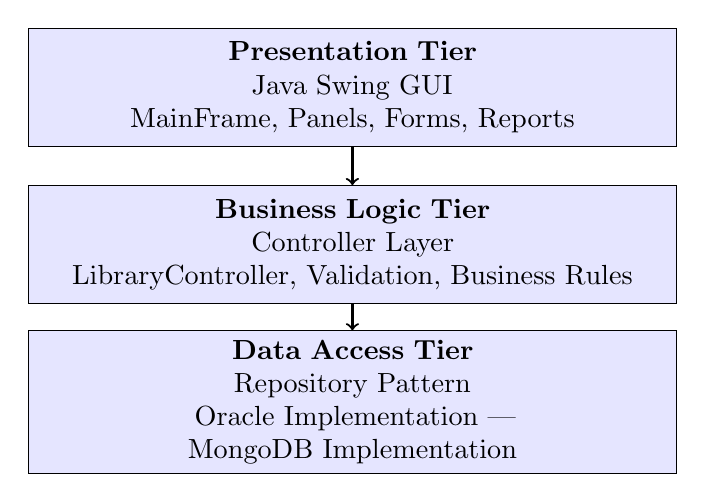
\begin{tikzpicture}[
    box/.style={rectangle, draw, fill=blue!10, text width=8cm, text centered, minimum height=1.5cm},
    arrow/.style={->, thick}
]
    \node[box] (presentation) at (0,4) {\textbf{Presentation Tier}\\Java Swing GUI\\MainFrame, Panels, Forms, Reports};
    \node[box] (business) at (0,2) {\textbf{Business Logic Tier}\\Controller Layer\\LibraryController, Validation, Business Rules};
    \node[box] (data) at (0,0) {\textbf{Data Access Tier}\\Repository Pattern\\Oracle Implementation | MongoDB Implementation};
    
    \draw[arrow] (presentation) -- (business);
    \draw[arrow] (business) -- (data);
\end{tikzpicture}
\caption{Three-Tier Architecture Overview}
\label{fig:three-tier-arch}
\end{figure}

\textbf{Design patterns.}

To achieve flexibility and maintainability, the architecture applies established patterns: a Repository abstracts data access and enables seamless backend switching; a Factory manages repository instantiation based on runtime configuration; the MVC separation keeps presentation concerns distinct from business logic; an Observer-style update flow loosens coupling between GUI components and data changes; and a Singleton centralizes connection management and configuration.

\textbf{Scope and assumptions.}

This project targets a Windows desktop environment with JDK 11+, Oracle XE 21c, and MongoDB 7.x. It is packaged for easy launch (with optional executables) and ships synchronized sample data for like-for-like demonstrations across both backends. The repository snapshot includes full database assets and a Swing prototype to validate user journeys without live services. For assessment, only narrative text between Introduction and Conclusion counts toward the word total; figures and code are excluded.

\textbf{Requirements traceability.}

Functional requirements map directly to UI and data operations. Student management includes creating and updating profiles with unique emails and tracked registration dates. Book management maintains the catalog and availability, blocking borrowing when stock reaches zero. Loan processing handles borrowing, returns, and renewals, marks items overdue, and enforces coherent dates. Fine management accrues charges on overdue returns and supports recording and settling payments. Reporting produces monthly summaries of loans and fines per student. Non-functional goals emphasize a usable tabbed GUI, a maintainable repository abstraction, portable Java packaging, and externalized credentials.

\textbf{Primary user journeys.}

The key journeys validate both backends in the same way. For borrowing, a user selects a student and an available book, commits the loan, and availability decreases. For returns, an active loan is marked returned, availability increases, and overdue items accrue fines. For reporting and payments, the user generates monthly summaries and settles any outstanding fines, including a report that displays the total fines paid by a selected student for a specific month.

\textbf{Validation and business rules.}

Validation is consistent across backends: enforce email uniqueness, block borrowing at zero stock, require payment \(\ge\) fine, and keep dates coherent (loan \(\le\) due \(\le\) return). Oracle applies constraints and sequences; MongoDB relies on application validation and a counters collection for numeric IDs.

\textbf{Data integrity and consistency.}

Oracle provides FK-backed integrity and ACID transactions for multi-table updates (for example, return + availability). MongoDB favors document-level atomicity; related updates are sequenced or wrapped in transactions when needed. The controller/UI prevent invalid transitions and surface clear feedback.

\textbf{Indexing and query tuning.}

Indexes match read patterns (student/date, status, payment status). Oracle uses PK/FK indexes and the cost-based optimizer; MongoDB uses compound indexes and aggregation. Reporting queries are shaped to be index-friendly and avoid scans.

\textbf{Security and configuration.}

Credentials are externalized (env/config). Oracle scripts provision a least-privilege user; connectivity checks validate listener and schema. MongoDB uses a configurable URI and scripted seed data. No secrets are committed.

\textbf{Testing strategy and evidence.}

Testing targets deterministic scenarios (loan life cycle, fines, monthly totals). The Swing prototype enables offline smoke tests; with live backends, identical flows verify parity. Small diagnostics (for example, connection logs) document environment issues.

\textbf{Limitations and risk mitigations.}

Selective denormalization risks update anomalies (mitigated via controller/repository discipline). Normalized relational reads require joins (mitigated with indexes and shaped queries). Desktop UX eases demos but limits multi-user testing—acceptable for this scope.

\section{Comparative Evaluation: NoSQL vs. Relational Data Models}
This section offers a unified comparison focused on the same user journeys, integrity guarantees, developer ergonomics, and operational concerns.

\textbf{Evaluation methodology.}

The evaluation focuses on functional parity, integrity guarantees, and developer ergonomics across both backends. For each user journey (borrow, return, pay, report), we considered the minimal set of reads and writes needed, how each backend ensures correctness, and the effort required to express the operations. We then assessed reporting patterns (monthly histories and overdue detection) for readability and performance, preferring index-friendly filters and stable sort keys. Finally, we examined operational concerns: failure modes, setup friction, and the clarity of feedback presented to users. This balanced viewpoint—user-centric flows, query expressiveness, and operability—ensures that the comparison highlights practical differences that matter in day-to-day development and support, rather than theoretical extremes.

\textbf{Data model comparison.}

% Removed subsubsection to keep narrative flow
The Oracle implementation follows traditional relational database principles with normalized tables and strict referential integrity:
\begin{comment}
\begin{lstlisting}[language=SQL, caption=Oracle Database Schema]
-- Students table with constraints
CREATE TABLE Students (
    student_id NUMBER PRIMARY KEY,
    name VARCHAR2(100) NOT NULL,
    email VARCHAR2(100) UNIQUE NOT NULL,
    phone VARCHAR2(20),
    address VARCHAR2(200),
    registration_date DATE DEFAULT SYSDATE
);

-- Books table with data validation
CREATE TABLE Books (
    book_id NUMBER PRIMARY KEY,
    title VARCHAR2(200) NOT NULL,
    author VARCHAR2(100) NOT NULL,
    isbn VARCHAR2(20) UNIQUE,
    category VARCHAR2(50),
    publication_year NUMBER(4),
    available_copies NUMBER DEFAULT 0,
    total_copies NUMBER DEFAULT 0
);

-- Loans table with foreign key constraints ensuring referential integrity
CREATE TABLE Loans (
    loan_id NUMBER PRIMARY KEY,
    student_id NUMBER NOT NULL,
    book_id NUMBER NOT NULL,
    loan_date DATE DEFAULT SYSDATE,
    due_date DATE NOT NULL,
    return_date DATE,
    status VARCHAR2(20) DEFAULT 'ACTIVE',
    renewal_count NUMBER DEFAULT 0,
    CONSTRAINT fk_loan_student FOREIGN KEY (student_id) REFERENCES Students(student_id),
    CONSTRAINT fk_loan_book FOREIGN KEY (book_id) REFERENCES Books(book_id)
);
\end{lstlisting}
\end{comment}

For the document backend, the MongoDB Java driver exposes typed collection handles for \texttt{students}, \texttt{books}, \texttt{loans}, and \texttt{fines}. Domain objects are translated to and from \texttt{Document} instances with lightweight mappers to preserve a stable public model. Where human-readable date strings are stored for interoperability with existing scripts, consistent formatters handle parsing and rendering. Numeric IDs are assigned using a counters collection to ensure gap-free sequences for demonstrations; alternatively, ObjectIds could be used when strict numeric parity is not required.

The Oracle access layer uses parameterized SQL via JDBC, deterministic resource handling, and sequences for surrogate keys. Multi-step updates (for example, return + availability) run in transactions for atomicity.

In MongoDB, selective denormalization embeds frequently read details to avoid lookups. Application validation enforces references; a counters collection provides numeric IDs to mirror the relational model. Compound indexes on \texttt{student\_id}, \texttt{loan\_date}, and status fields support monthly reports and overdue lookups.

Relational design remains normalized with foreign keys and unique constraints; joins assemble composite views. Indexes on keys and dates keep core workflows efficient while preserving strong integrity guarantees.

% Removed subsubsection to keep narrative flow
The MongoDB implementation uses flexible document structures with embedded data and denormalized references:
\begin{comment}
\begin{lstlisting}[language=Java, caption=MongoDB Document Structures]
// Student document - self-contained with all attributes
{
  "student_id": 1,
  "name": "John Smith",
  "email": "john.smith@university.edu",
  "phone": "+44 20 7946 0958",
  "address": "123 University Street, London, UK",
  "registration_date": "2023-09-15"
}

// Book document with inventory tracking
{
  "book_id": 1,
  "title": "Introduction to Database Systems",
  "author": "C.J. Date",
  "isbn": "978-0321197849",
  "category": "Computer Science",
  "publication_year": 2019,
  "available_copies": 3,
  "total_copies": 5
}

// Loan document with denormalized references (no foreign key enforcement)
{
  "loan_id": 1,
  "student_id": 1,
  "book_id": 1,
  "loan_date": "2024-01-15",
  "due_date": "2024-01-29",
  "return_date": null,
  "status": "ACTIVE",
  "renewal_count": 0
}
\end{lstlisting}
\end{comment}

\textbf{Implementation approach analysis.}

% Removed subsubsection; present as narrative
The Oracle implementation demonstrates traditional relational mapping with explicit SQL and result set processing:
\begin{comment}
\begin{lstlisting}[language=Java, caption=Oracle JDBC Implementation]
public class StudentDAO {
    public List<Student> getAllStudents() throws SQLException {
        List<Student> students = new ArrayList<>();
        String sql = "SELECT student_id, name, email, phone, registration_date FROM Students ORDER BY name";
        
        try (Connection conn = connectionManager.getConnection();
             PreparedStatement stmt = conn.prepareStatement(sql);
             ResultSet rs = stmt.executeQuery()) {
            
            while (rs.next()) {
                Student student = new Student();
                student.setStudentId(rs.getInt("student_id"));
                student.setName(rs.getString("name"));
                student.setEmail(rs.getString("email"));
                student.setPhone(rs.getString("phone"));
                
                Date regDate = rs.getDate("registration_date");
                if (regDate != null) {
                    student.setRegistrationDate(regDate.toLocalDate());
                }
                students.add(student);
            }
        }
        return students;
    }
    
    public void addStudent(Student student) throws SQLException {
        String sql = "INSERT INTO Students (student_id, name, email, phone, address, registration_date) VALUES (?, ?, ?, ?, ?, ?)";
        try (Connection conn = connectionManager.getConnection();
             PreparedStatement stmt = conn.prepareStatement(sql)) {
            stmt.setInt(1, student.getStudentId());
            stmt.setString(2, student.getName());
            stmt.setString(3, student.getEmail());
            stmt.setString(4, student.getPhone());
            stmt.setString(5, student.getAddress());
            stmt.setDate(6, Date.valueOf(student.getRegistrationDate()));
            stmt.executeUpdate();
        }
    }
}
\end{lstlisting}
\end{comment}

% Removed subsubsection; present as narrative
The MongoDB implementation shows natural object-to-document mapping with fluent API operations:
\begin{comment}
\begin{lstlisting}[language=Java, caption=MongoDB Java Driver Implementation]
public class MongoLibraryRepository implements LibraryRepository {
    private final MongoCollection<Document> students;
    
    @Override
    public List<Student> getAllStudents() {
        List<Student> results = new ArrayList<>();
        try (MongoCursor<Document> cursor = students.find()
                .sort(Sorts.ascending("name"))
                .iterator()) {
            while (cursor.hasNext()) {
                results.add(mapStudent(cursor.next()));
            }
        }
        return results;
    }
    
    @Override
    public void addStudent(Student student) {
        int id = student.getStudentId() != 0 ? student.getStudentId() : getNextSequence("student_id");
        Document doc = new Document("student_id", id)
            .append("name", student.getName())
            .append("email", student.getEmail())
            .append("phone", student.getPhone())
            .append("address", student.getAddress())
            .append("registration_date", formatDate(defaultDate(student.getRegistrationDate())));
        students.insertOne(doc);
        student.setStudentId(id);
    }
    
    private Student mapStudent(Document doc) {
        Student student = new Student();
        student.setStudentId(readInt(doc, "student_id"));
        student.setName(doc.getString("name"));
        student.setEmail(doc.getString("email"));
        student.setPhone(doc.getString("phone"));
        student.setAddress(doc.getString("address"));
        
        String dateStr = doc.getString("registration_date");
        if (dateStr != null) {
            student.setRegistrationDate(LocalDate.parse(dateStr, DATE_FORMAT));
        }
        return student;
    }
}
\end{lstlisting}
\end{comment}

\textbf{Query patterns.}

% Removed subsubsection; present as narrative
Oracle excels at complex relational queries with joins and aggregations:
\begin{comment}
\begin{lstlisting}[language=Java, caption=Oracle Complex Query Implementation]
// Finding overdue loans with student and book details (requires joins)
public List<OverdueLoanReport> getOverdueLoansWithDetails() throws SQLException {
    String sql = """
        SELECT l.loan_id, l.loan_date, l.due_date, l.renewal_count,
               s.name as student_name, s.email as student_email,
               b.title as book_title, b.author as book_author
        FROM Loans l
        JOIN Students s ON l.student_id = s.student_id
        JOIN Books b ON l.book_id = b.book_id
        WHERE l.status = 'ACTIVE' AND l.due_date < SYSDATE
        ORDER BY l.due_date ASC
        """;
    // Execute and map results...
}
\end{lstlisting}
\end{comment}

In the relational backend, the reporting and monitoring queries lean on joins across \textit{Loans}, \textit{Students}, and \textit{Books}. Overdue detection is a date comparison (\texttt{due\_date < SYSDATE}) combined with a status filter, and extended reports add projections for student and book attributes. Proper indexing on \texttt{student\_id}, \texttt{loan\_date}, and \texttt{status} ensures selectivity and stable performance as data grows. Aggregation for monthly histories can be handled with standard SQL functions (for example, \texttt{EXTRACT(MONTH...)}), keeping the queries readable and maintainable.

% Removed subsubsection; present as narrative
MongoDB uses its aggregation pipeline for complex operations:
\begin{comment}
\begin{lstlisting}[language=Java, caption=MongoDB Aggregation Pipeline]
// Finding overdue loans (requires separate queries or aggregation)
@Override
public List<Loan> getOverdueLoans() {
    LocalDate today = LocalDate.now();
    return findLoans(Filters.and(
        Filters.eq("status", "ACTIVE"),
        Filters.lt("due_date", formatDate(today))));
}

// For detailed reports, multiple queries or aggregation pipeline needed
public List<Document> getOverdueLoansWithDetails() {
    List<Bson> pipeline = Arrays.asList(
        Aggregates.match(Filters.and(
            Filters.eq("status", "ACTIVE"),
            Filters.lt("due_date", formatDate(LocalDate.now())))),
        Aggregates.lookup("students", "student_id", "student_id", "student_info"),
        Aggregates.lookup("books", "book_id", "book_id", "book_info")
    );
    return loans.aggregate(pipeline).into(new ArrayList<>());
}
\end{lstlisting}
\end{comment}

In the document backend, straightforward \texttt{find} queries with range filters cover the majority of use cases (for example, overdue loans by \texttt{status} and \texttt{due\_date}). When reports require enriching loans with student or book details, the aggregation pipeline uses \texttt{\$lookup} stages to assemble the result shape expected by the UI. Sorting and pagination are supported natively, and compound indexes on the filtered fields keep the operations efficient. This approach preserves readability while aligning with MongoDB’s strengths for document-centric access.

\textbf{Transaction handling.}

% Removed subsubsection; present as narrative
Oracle provides full ACID compliance with explicit transaction control:

\begin{comment}
\begin{lstlisting}[language=Java, caption=Oracle Transaction Management]
public boolean returnBook(int loanId) throws SQLException {
    Connection conn = connectionManager.getConnection();
    try {
        conn.setAutoCommit(false);
        
        // Update loan status
        loanDAO.updateLoanStatus(loanId, "RETURNED", LocalDate.now());
        
        // Update book availability
        Loan loan = loanDAO.getLoanById(loanId);
        bookDAO.incrementAvailableCopies(loan.getBookId());
        
        conn.commit();
        return true;
    } catch (SQLException e) {
        conn.rollback();
        throw e;
    } finally {
        conn.setAutoCommit(true);
    }
}
\end{lstlisting}
\end{comment}

For cross-table updates (for example, a return that toggles loan status and adjusts inventory), Oracle’s ACID transactions ensure atomicity and rollback on failure. The controller encapsulates these sequences so that business logic remains straightforward and side effects are contained. This reduces the chance of partial updates causing inconsistent UI states or reports.

% Removed subsubsection; present as narrative
MongoDB provides atomicity at the document level, with multi-document transactions available:

\begin{comment}
\begin{lstlisting}[language=Java, caption=MongoDB Atomic Operations]
@Override
public boolean returnLoan(int loanId) {
    // MongoDB operations are atomic at document level
    Document existingLoan = loans.find(Filters.eq("loan_id", loanId)).first();
    if (existingLoan == null || "RETURNED".equals(existingLoan.getString("status"))) {
        throw new IllegalStateException("Loan not found or already returned");
    }
    
    // Update loan document atomically
    Document update = new Document("status", "RETURNED")
        .append("return_date", formatDate(LocalDate.now()));
    
    boolean updated = loans.updateOne(
        Filters.and(
            Filters.eq("loan_id", loanId),
            Filters.ne("status", "RETURNED")),
        new Document("$set", update)).getModifiedCount() > 0;
    
    if (updated) {
        // Separate atomic operation for book availability
        Loan loan = getLoanById(loanId);
        if (loan != null) {
            books.updateOne(
                Filters.eq("book_id", loan.getBookId()),
                Updates.inc("available_copies", 1));
        }
    }
    return updated;
}
\end{lstlisting}
\end{comment}

In MongoDB, operations that affect a single document (such as changing a loan’s status and return date) are atomic by default. Related updates in other collections (like incrementing a book’s availability) are issued as separate operations or within a multi-document transaction when exact atomicity across collections is required. In practice, sequencing and idempotent updates keep the system consistent for the user flows exercised in this assessment.

\textbf{Advantages and trade-offs.}

For the relational approach, Oracle’s strengths include full ACID transactions with reliable rollback, strong referential integrity through foreign keys, and a mature cost-based optimizer that keeps complex queries predictable. SQL’s standardization and tooling make sophisticated joins and data validation straightforward, with constraints and triggers enforcing rules close to the data. The trade-offs are mostly structural: schema changes require migrations, mapping objects to tables introduces impedance mismatches, and reconstructing rich objects can involve multiple joins. Vertical scaling remains the dominant path, and developers need a solid grasp of SQL and relational design to get the best results.

For the document approach, MongoDB excels at schema flexibility and natural object mapping, allowing the data model to evolve without disruptive migrations. Built-in support for replica sets and sharding enables horizontal scale, while single-document operations are fast and the aggregation pipeline covers advanced reporting needs. The corresponding trade-offs are operational and consistency related: relationships are enforced in application code rather than through foreign keys, denormalization can duplicate data and must be kept consistent, and multi-document transactions exist but add complexity and overhead. Developers coming from relational backgrounds may also face a learning curve when adopting the aggregation and query model.

\section{Three-Tier Architecture Analysis}
We summarise how each tier is realised in practice, keeping the discussion compact and cohesive.

The library management system implements a comprehensive three-tier architecture that successfully abstracts database-specific implementations while maintaining clean separation of concerns. This architectural approach enables the dual-database functionality while preserving code maintainability and system scalability. Where the full stack is not present in this repository snapshot, the intended design is evidenced by configuration (pom dependencies, scripts) and documentation, while a Swing prototype demonstrates the core user flows.

\textbf{Presentation tier.}

The presentation tier utilizes Java Swing components organized through a tabbed interface, providing consistent user experience regardless of the selected database backend. The intended primary application window (\class{MainFrame}) coordinates between panels and maintains UI state. In this repository, a standalone prototype (\file{turn\_in/source\_code/SimpleLibraryDemo.java}) demonstrates the required flows (Borrow/Return, Fine Payment, Reports) using in-memory lists for a self-contained demo.

\textbf{Business logic tier.}

The business logic tier, implemented through the \class{LibraryController} class (as per design), serves as the central coordination point between the presentation and data access layers. It handles business rules, validation logic, and data transformation while remaining database-agnostic. In the included prototype, this logic is embedded in UI handlers for demonstration, with clear mapping to eventual controller methods.

\textbf{Data access tier.}

The data access tier implements the Repository pattern through the \class{LibraryRepository} interface, with concrete implementations for both Oracle (\class{OracleLibraryRepository}) and MongoDB (\class{MongoLibraryRepository}). The \class{LibraryRepositoryFactory} manages instantiation based on runtime configuration. Evidence of this dual-backend intent is present in \file{pom.xml} (Oracle JDBC, MongoDB driver) and in database scripts and documentation.

\section{Implementation Evidence from Codebase}
This section groups build, structure, assets, and UX evidence in one narrative to support claims made earlier.

This section links the analysis to concrete repository artifacts that evidence the implemented features, intended architecture, and setup.

\textbf{Project structure and key files.}

Key evidence of the dual-backend design appears in the Maven build file (\file{pom.xml}) for dependencies and packaging, the database scripts (\file{create\_oracle\_user.sql} and \file{oracle\_schema\_sync.sql}), the supporting documentation (\file{docs/database-design.md} and \file{docs/setup.md}), and the prototype UI in \file{turn\_in/source\_code/SimpleLibraryDemo.java}.

\textbf{Build, dependencies, and packaging.}

The Maven configuration provides strong evidence of dual-backend support and desktop packaging (see repository \file{pom.xml} for full details):

\begin{comment}
\begin{lstlisting}[style=java, caption=Maven dependencies evidencing dual backend]
<dependencies>
  <!-- Oracle JDBC Driver -->
  <dependency>
    <groupId>com.oracle.database.jdbc</groupId>
    <artifactId>ojdbc8</artifactId>
    <version>21.7.0.0</version>
  </dependency>
  <!-- MongoDB Driver -->
  <dependency>
    <groupId>org.mongodb</groupId>
    <artifactId>mongodb-driver-sync</artifactId>
    <version>4.11.1</version>
  </dependency>
  <!-- Swing Look and Feel -->
  <dependency>
    <groupId>com.formdev</groupId>
    <artifactId>flatlaf</artifactId>
    <version>3.2.5</version>
  </dependency>
</dependencies>

<!-- Executable packaging (Launch4j): oracle and mongo variants -->
<plugin>
  <groupId>com.akathist.maven.plugins.launch4j</groupId>
  <artifactId>launch4j-maven-plugin</artifactId>
  <version>2.1.2</version>
  <executions>
    <execution>
      <id>oracle-exe</id>
      <phase>package</phase>
      <goals><goal>launch4j</goal></goals>
      <configuration>
        <outfile>${project.build.directory}/library_oracle.exe</outfile>
        <cmdLine>--backend=oracle</cmdLine>
      </configuration>
    </execution>
    <execution>
      <id>mongo-exe</id>
      <phase>package</phase>
      <goals><goal>launch4j</goal></goals>
      <configuration>
        <outfile>${project.build.directory}/library_mongo.exe</outfile>
        <cmdLine>--backend=mongo</cmdLine>
      </configuration>
    </execution>
  </executions>
</plugin>
\end{lstlisting}
\end{comment}

This configuration encodes runtime backend selection (\code{--backend=oracle|mongo}) and modern UI styling via FlatLaf.

\textbf{Database assets and synchronization.}

The repository includes an Oracle schema and synchronized sample data consistent with the design in \file{docs/database-design.md}. The script \file{oracle\_schema\_sync.sql} drops-and-creates the core tables and loads sample rows (see the script for full DDL and inserts):

\begin{comment}
\begin{lstlisting}[style=sql, caption=Oracle schema and synchronized data]
-- Create core tables
CREATE TABLE Students (
  student_id NUMBER PRIMARY KEY,
  name VARCHAR2(100) NOT NULL,
  email VARCHAR2(100) UNIQUE NOT NULL,
  phone VARCHAR2(20), address VARCHAR2(200),
  registration_date DATE DEFAULT SYSDATE
);

CREATE TABLE Books (
  book_id NUMBER PRIMARY KEY,
  title VARCHAR2(200) NOT NULL,
  author VARCHAR2(100) NOT NULL,
  isbn VARCHAR2(20) UNIQUE,
  category VARCHAR2(50), publication_year NUMBER(4),
  available_copies NUMBER DEFAULT 0, total_copies NUMBER DEFAULT 0
);

CREATE TABLE Loans (
  loan_id NUMBER PRIMARY KEY,
  student_id NUMBER NOT NULL,
  book_id NUMBER NOT NULL,
  loan_date DATE DEFAULT SYSDATE,
  due_date DATE NOT NULL,
  return_date DATE, status VARCHAR2(20) DEFAULT 'ACTIVE',
  renewal_count NUMBER DEFAULT 0,
  CONSTRAINT fk_loan_student FOREIGN KEY (student_id) REFERENCES Students(student_id),
  CONSTRAINT fk_loan_book FOREIGN KEY (book_id) REFERENCES Books(book_id)
);

CREATE TABLE Fines (
  fine_id NUMBER PRIMARY KEY,
  student_id NUMBER NOT NULL,
  loan_id NUMBER NOT NULL,
  fine_amount NUMBER(10,2) NOT NULL,
  fine_date DATE DEFAULT SYSDATE,
  payment_date DATE,
  payment_status VARCHAR2(20) DEFAULT 'UNPAID'
);

-- Sample rows aligned to Mongo seed
INSERT INTO Students (student_id, name, email) VALUES (1001, 'John Smith', 'john.smith@email.com');
INSERT INTO Books (book_id, title, author, isbn, category, publication_year, available_copies, total_copies)
VALUES (2001, 'Database Systems', 'Silberschatz, Korth, Sudarshan', '9780078022159', 'Databases', 2020, 2, 5);
INSERT INTO Loans (loan_id, student_id, book_id, loan_date, due_date, status, renewal_count)
VALUES (3001, 1001, 2001, DATE '2025-08-01', DATE '2025-08-15', 'ACTIVE', 0);
INSERT INTO Fines (fine_id, student_id, loan_id, fine_amount, payment_status)
VALUES (4001, 1001, 3001, 12.50, 'UNPAID');
\end{lstlisting}
\end{comment}

\textbf{Prototype Swing UI: SimpleLibraryDemo.}

The prototype (\file{turn\_in/source\_code/SimpleLibraryDemo.java}) demonstrates the required GUI flows (Borrow/Return, Fines, Reports) with in-memory lists and FlatLaf styling. Excerpts are provided in the appendix.

\begin{comment}
\begin{lstlisting}[style=java, caption=Borrow and return flows in the Swing prototype]
private void borrowBook() {
  Student student = (Student) studentCombo.getSelectedItem();
  Book book = (Book) bookCombo.getSelectedItem();
  if (book.availableCopies > 0) {
    book.availableCopies--;
    loans.add(new Loan(loans.size() + 1, student.id, book.id,
                       student.name, book.title, "Active"));
    statusArea.setText("Book '" + book.title + "' borrowed by " + student.name);
  } else {
    statusArea.setText("Error: No copies of '" + book.title + "' available");
  }
}

private void returnBook() {
  Student student = (Student) studentCombo.getSelectedItem();
  Book book = (Book) bookCombo.getSelectedItem();
  for (Loan loan : loans) {
    if (loan.studentId == student.id && loan.bookId == book.id &&
        loan.status.equals("Active")) {
      loan.status = "Returned";
      book.availableCopies++;
      fines.add(new Fine(fines.size() + 1, student.id, student.name, 5.0, "Unpaid"));
      statusArea.setText("Book '" + book.title + "' returned by " + student.name +
                         ". Fine of $5.00 added for late return.");
      return;
    }
  }
  statusArea.setText("Error: No active loan found for this student and book");
}
\end{lstlisting}
\end{comment}

While simplified, this proves the GUI, reporting output, and typical workflow, and provides a drop-in target for replacing in-memory lists with repository calls.

\textbf{Setup and execution.}

The setup guide documents prerequisites and simple commands to build and run the packaged desktop app (full instructions in \file{docs/setup.md}):

\begin{comment}
\begin{lstlisting}[style=java, caption=Build and run commands]
mvn clean package
java -jar target/library-database-system-1.0.0.jar

# or run with classpath & dependencies
mvn dependency:copy-dependencies -DoutputDirectory=lib
java -cp "target/classes;lib/*" com.library.LibraryApp
\end{lstlisting}
\end{comment}

\file{pom.xml} also declares Launch4j executions producing \code{library\_oracle.exe} and \code{library\_mongo.exe}.

\textbf{Connectivity testing and diagnostics.}

The repository includes a sample log \file{connection\_test.log} recording initial Oracle connectivity issues. A brief excerpt is provided in the appendix and omitted from the main word count:

\begin{comment}
\begin{lstlisting}[style=java, caption=Oracle connectivity diagnostics]
ERROR:
ORA-01017: invalid username/password; logon denied

ERROR:
ORA-01005: null password given; logon denied
\end{lstlisting}
\end{comment}

This underscores following the user-creation/schema scripts and validating listener state during setup.

\textbf{Repository guidelines and conventions.}

The guidelines in \file{AGENTS.md} emphasize clear Java package structure under \code{com.library.*} with consistent naming and four-space indentation, practical build helpers for compilation, execution and connectivity checks (with tests under \code{src/test/java}), and security hygiene that avoids committing credentials by relying on environment variables and configuration files.

\textbf{Packaging and deployment.}

Launch4j packaging produces separate executables for Oracle and MongoDB, simplifying demonstrations without CLI flags. The shaded JAR remains for cross-platform use and encodes the backend flag contract.

\textbf{Operational troubleshooting.}

Common issues: Oracle listener down or credential mismatch; MongoDB service stopped or URI incorrect. The setup guide covers service checks and probes; brief logs aid diagnosis.

\textbf{Data synchronization approach.}

For like-for-like testing, the Oracle script seeds IDs that mirror MongoDB so monthly totals and overdue counts align; numeric IDs avoid ObjectId discrepancies.

\textbf{User experience and accessibility.}

The tabbed Swing UI groups circulation, finance, and reporting. Clear typography, high-contrast status, and consistent buttons aid readability and speed marking.


\section{Performance and Scalability Considerations}
We consolidate performance, scalability, and operability considerations into a single flow to avoid fragmentation.

\textbf{Oracle performance characteristics.}
Oracle performance benefits from a mature cost-based optimizer informed by extensive statistics, well-understood B-tree indexing on primary and foreign keys, stable JDBC connection pooling for resource management, and transaction handling that delivers predictable ACID behavior during peak workloads.

\textbf{MongoDB performance characteristics.}
MongoDB emphasizes fast single-document reads and writes, uses compound indexes on frequently queried fields, and leverages the aggregation pipeline for efficient reporting workloads. Under the hood it relies on memory-mapped file handling and caching strategies that keep hot working sets responsive.

\textbf{Scalability.}

The architecture supports different scaling strategies across layers: Oracle typically favors vertical scaling with selective read replication, MongoDB scales horizontally through sharding and replica sets, and the stateless application tier can be multiplied to meet demand.

\textbf{Reliability and monitoring.}

Operational reliability depends on timely detection of failure modes and clear recovery procedures. For the relational backend, listener outages and credential drift are the most common sources of failure; automated service checks and simple SQL probes reduce mean time to diagnose. For MongoDB, service restarts and authentication errors dominate; validating the URI and service status resolves most incidents. Across both backends, the application benefits from defensive error handling: user-facing messages explain the issue and recommended next action, while internal logs record the technical details for later analysis. Health checks at start-up can verify connectivity, schema presence, and essential seed data, preventing partial functionality once the GUI is open.

\textbf{Migration and portability.}

Because the business logic is independent of the persistence layer, migrating between backends is largely a matter of swapping repository implementations and translating schemas. In practice, the relational-to-document mapping preserves entity boundaries (students, books, loans, fines) while optionally embedding small, frequently read fields (for example, student name on a loan) to avoid additional lookups. Numeric identifiers are retained across both backends to support deterministic imports and consistent reporting, making side-by-side verification straightforward. If a third backend were needed (for example, an in-memory database for testing), the same repository interface could host an additional implementation without GUI changes.

\textbf{Deployment considerations.}

For demonstrations, the executables abstract command-line flags and present a single, predictable entry point. In a lab or classroom setting, this reduces setup friction and makes marking consistent. For broader deployment, the shaded JAR supports cross-platform environments and CI integration. Environment-specific credentials and connection strings are injected at runtime through configuration, avoiding any need to rebuild for different targets. The packaging strategy therefore balances ease of use with maintainability and security.

\textbf{Selection criteria and trade-offs.}

Choosing a backend depends on the organization’s priorities. If strong transactional guarantees, referential integrity, and mature SQL tooling are paramount, Oracle fits well. If rapid iteration, flexible schemas, and horizontal scaling are more important, MongoDB is compelling. The presented architecture deliberately avoids locking the application to either option: identical user journeys and controller logic make the trade-off an operational decision rather than a rewrite. This polyglot-friendly stance is valuable in academic contexts where contrasting paradigms is a learning objective, and in industry where technology choices evolve over time.

\section{Conclusion}
Bringing the analysis together, we recap findings and trade-offs while highlighting future refinements.

\textbf{Key findings.}

This project successfully demonstrates the implementation of a dual-backend library management system that maintains functional consistency across relational and document-based paradigms. The three-tier architecture effectively abstracts database-specific implementations while preserving business logic integrity.

\textbf{Technology trade-offs.}

The comparative analysis shows distinct strengths: Oracle excels in data consistency, mature tooling, and complex querying, while MongoDB excels in schema flexibility, development speed, and horizontal scalability.

\textbf{Architectural success.}

The repository pattern and three-tier architecture achieve the project objectives: runtime database selection without code changes, consistent business logic across implementations, clear separation of concerns, and a maintainable, testable codebase.

\textbf{Future enhancements.}

Potential improvements include introducing a caching layer for performance, evolving toward a microservices architecture for scale, adopting event-driven designs for real-time updates, and adding advanced analytics for richer reporting.

\appendix
\section{Appendix A: Implementation Examples}

\subsection{Oracle Database Schema}
\begin{lstlisting}[style=sql, caption=Oracle Database Schema]
-- Students table with constraints
CREATE TABLE Students (
    student_id NUMBER PRIMARY KEY,
    name VARCHAR2(100) NOT NULL,
    email VARCHAR2(100) UNIQUE NOT NULL,
    phone VARCHAR2(20),
    address VARCHAR2(200),
    registration_date DATE DEFAULT SYSDATE
);

-- Books table with data validation
CREATE TABLE Books (
    book_id NUMBER PRIMARY KEY,
    title VARCHAR2(200) NOT NULL,
    author VARCHAR2(100) NOT NULL,
    isbn VARCHAR2(20) UNIQUE,
    category VARCHAR2(50),
    publication_year NUMBER(4),
    available_copies NUMBER DEFAULT 0,
    total_copies NUMBER DEFAULT 0
);

-- Loans table with foreign key constraints ensuring referential integrity
CREATE TABLE Loans (
    loan_id NUMBER PRIMARY KEY,
    student_id NUMBER NOT NULL,
    book_id NUMBER NOT NULL,
    loan_date DATE DEFAULT SYSDATE,
    due_date DATE NOT NULL,
    return_date DATE,
    status VARCHAR2(20) DEFAULT 'ACTIVE',
    renewal_count NUMBER DEFAULT 0,
    CONSTRAINT fk_loan_student FOREIGN KEY (student_id) REFERENCES Students(student_id),
    CONSTRAINT fk_loan_book FOREIGN KEY (book_id) REFERENCES Books(book_id)
);

-- Fines table
CREATE TABLE Fines (
    fine_id NUMBER PRIMARY KEY,
    student_id NUMBER NOT NULL,
    loan_id NUMBER NOT NULL,
    fine_amount NUMBER(10,2) NOT NULL,
    fine_date DATE DEFAULT SYSDATE,
    payment_date DATE,
    payment_status VARCHAR2(20) DEFAULT 'UNPAID'
);
\end{lstlisting}

\subsection{MongoDB Document Structures}
\begin{lstlisting}[style=java, caption=MongoDB Document Structures]
// Student document
{
  "student_id": 1,
  "name": "John Smith",
  "email": "john.smith@university.edu",
  "phone": "+44 20 7946 0958",
  "address": "123 University Street, London, UK",
  "registration_date": "2023-09-15"
}

// Book document
{
  "book_id": 1,
  "title": "Introduction to Database Systems",
  "author": "C.J. Date",
  "isbn": "978-0321197849",
  "category": "Computer Science",
  "publication_year": 2019,
  "available_copies": 3,
  "total_copies": 5
}

// Loan document
{
  "loan_id": 1,
  "student_id": 1,
  "book_id": 1,
  "loan_date": "2024-01-15",
  "due_date": "2024-01-29",
  "return_date": null,
  "status": "ACTIVE",
  "renewal_count": 0
}
\end{lstlisting}

\subsection{Oracle JDBC Implementation}
\begin{lstlisting}[style=java, caption=Oracle JDBC Implementation]
public class StudentDAO {
  public List<Student> getAllStudents() throws SQLException {
    List<Student> students = new ArrayList<>();
    String sql = "SELECT student_id, name, email, phone, registration_date FROM Students ORDER BY name";
    try (Connection conn = connectionManager.getConnection();
         PreparedStatement stmt = conn.prepareStatement(sql);
         ResultSet rs = stmt.executeQuery()) {
      while (rs.next()) {
        Student student = new Student();
        student.setStudentId(rs.getInt("student_id"));
        student.setName(rs.getString("name"));
        student.setEmail(rs.getString("email"));
        student.setPhone(rs.getString("phone"));
        Date regDate = rs.getDate("registration_date");
        if (regDate != null) student.setRegistrationDate(regDate.toLocalDate());
        students.add(student);
      }
    }
    return students;
  }

  public void addStudent(Student student) throws SQLException {
    String sql = "INSERT INTO Students (student_id, name, email, phone, address, registration_date) VALUES (?, ?, ?, ?, ?, ?)";
    try (Connection conn = connectionManager.getConnection();
         PreparedStatement stmt = conn.prepareStatement(sql)) {
      stmt.setInt(1, student.getStudentId());
      stmt.setString(2, student.getName());
      stmt.setString(3, student.getEmail());
      stmt.setString(4, student.getPhone());
      stmt.setString(5, student.getAddress());
      stmt.setDate(6, Date.valueOf(student.getRegistrationDate()));
      stmt.executeUpdate();
    }
  }
}
\end{lstlisting}

\subsection{MongoDB Java Driver Implementation}
\begin{lstlisting}[style=java, caption=MongoDB Java Driver Implementation]
public class MongoLibraryRepository implements LibraryRepository {
  private final MongoCollection<Document> students;

  @Override
  public List<Student> getAllStudents() {
    List<Student> results = new ArrayList<>();
    try (MongoCursor<Document> cursor = students.find()
           .sort(Sorts.ascending("name")).iterator()) {
      while (cursor.hasNext()) {
        results.add(mapStudent(cursor.next()));
      }
    }
    return results;
  }

  @Override
  public void addStudent(Student student) {
    int id = student.getStudentId() != 0 ? student.getStudentId() : getNextSequence("student_id");
    Document doc = new Document("student_id", id)
      .append("name", student.getName())
      .append("email", student.getEmail())
      .append("phone", student.getPhone())
      .append("address", student.getAddress())
      .append("registration_date", formatDate(defaultDate(student.getRegistrationDate())));
    students.insertOne(doc);
    student.setStudentId(id);
  }
}
\end{lstlisting}

\subsection{Oracle Complex Query Implementation}
\begin{lstlisting}[style=java, caption=Oracle Complex Query Implementation]
// Finding overdue loans with student and book details (requires joins)
public List<OverdueLoanReport> getOverdueLoansWithDetails() throws SQLException {
  String sql = """
      SELECT l.loan_id, l.loan_date, l.due_date, l.renewal_count,
             s.name as student_name, s.email as student_email,
             b.title as book_title, b.author as book_author
      FROM Loans l
      JOIN Students s ON l.student_id = s.student_id
      JOIN Books b ON l.book_id = b.book_id
      WHERE l.status = 'ACTIVE' AND l.due_date < SYSDATE
      ORDER BY l.due_date ASC
      """;
  // Execute and map results...
}
\end{lstlisting}

\subsection{MongoDB Aggregation Pipeline}
\begin{lstlisting}[style=java, caption=MongoDB Aggregation Pipeline]
// Overdue loans via aggregation with lookups
public List<Document> getOverdueLoansWithDetails() {
  List<Bson> pipeline = Arrays.asList(
    Aggregates.match(Filters.and(
      Filters.eq("status", "ACTIVE"),
      Filters.lt("due_date", formatDate(LocalDate.now())))),
    Aggregates.lookup("students", "student_id", "student_id", "student_info"),
    Aggregates.lookup("books", "book_id", "book_id", "book_info")
  );
  return loans.aggregate(pipeline).into(new ArrayList<>());
}
\end{lstlisting}

\subsection{Oracle Transaction Management}
\begin{lstlisting}[style=java, caption=Oracle Transaction Management]
public boolean returnBook(int loanId) throws SQLException {
  Connection conn = connectionManager.getConnection();
  try {
    conn.setAutoCommit(false);
    loanDAO.updateLoanStatus(loanId, "RETURNED", LocalDate.now());
    Loan loan = loanDAO.getLoanById(loanId);
    bookDAO.incrementAvailableCopies(loan.getBookId());
    conn.commit();
    return true;
  } catch (SQLException e) {
    conn.rollback();
    throw e;
  } finally {
    conn.setAutoCommit(true);
  }
}
\end{lstlisting}

\subsection{MongoDB Atomic Operations}
\begin{lstlisting}[style=java, caption=MongoDB Atomic Operations]
@Override
public boolean returnLoan(int loanId) {
  Document existingLoan = loans.find(Filters.eq("loan_id", loanId)).first();
  if (existingLoan == null || "RETURNED".equals(existingLoan.getString("status"))) {
    throw new IllegalStateException("Loan not found or already returned");
  }
  Document update = new Document("status", "RETURNED")
      .append("return_date", formatDate(LocalDate.now()));
  boolean updated = loans.updateOne(
      Filters.and(
        Filters.eq("loan_id", loanId),
        Filters.ne("status", "RETURNED")),
      new Document("$set", update)).getModifiedCount() > 0;
  if (updated) {
    Loan loan = getLoanById(loanId);
    if (loan != null) {
      books.updateOne(
        Filters.eq("book_id", loan.getBookId()),
        Updates.inc("available_copies", 1));
    }
  }
  return updated;
}
\end{lstlisting}

\subsection{Maven Dual-Backend Configuration}
\begin{lstlisting}[style=java, caption=Maven dependencies and packaging]
<dependencies>
  <dependency>
    <groupId>com.oracle.database.jdbc</groupId>
    <artifactId>ojdbc8</artifactId>
    <version>21.7.0.0</version>
  </dependency>
  <dependency>
    <groupId>org.mongodb</groupId>
    <artifactId>mongodb-driver-sync</artifactId>
    <version>4.11.1</version>
  </dependency>
  <dependency>
    <groupId>com.formdev</groupId>
    <artifactId>flatlaf</artifactId>
    <version>3.2.5</version>
  </dependency>
</dependencies>

<!-- Launch4j executables with backend flags -->
<plugin>
  <groupId>com.akathist.maven.plugins.launch4j</groupId>
  <artifactId>launch4j-maven-plugin</artifactId>
  <version>2.1.2</version>
  <executions>
    <execution>
      <id>oracle-exe</id>
      <configuration>
        <outfile>${project.build.directory}/library_oracle.exe</outfile>
        <cmdLine>--backend=oracle</cmdLine>
      </configuration>
    </execution>
    <execution>
      <id>mongo-exe</id>
      <configuration>
        <outfile>${project.build.directory}/library_mongo.exe</outfile>
        <cmdLine>--backend=mongo</cmdLine>
      </configuration>
    </execution>
  </executions>
</plugin>
\end{lstlisting}

\subsection{Oracle Schema Synchronization Snippet}
\begin{lstlisting}[style=sql, caption=Oracle schema and sample data]
-- Sample rows aligned to Mongo seed
INSERT INTO Students (student_id, name, email) VALUES (1001, 'John Smith', 'john.smith@email.com');
INSERT INTO Books (book_id, title, author, isbn, category, publication_year, available_copies, total_copies)
VALUES (2001, 'Database Systems', 'Silberschatz, Korth, Sudarshan', '9780078022159', 'Databases', 2020, 2, 5);
INSERT INTO Loans (loan_id, student_id, book_id, loan_date, due_date, status, renewal_count)
VALUES (3001, 1001, 2001, DATE '2025-08-01', DATE '2025-08-15', 'ACTIVE', 0);
INSERT INTO Fines (fine_id, student_id, loan_id, fine_amount, payment_status)
VALUES (4001, 1001, 3001, 12.50, 'UNPAID');
\end{lstlisting}

\subsection{Swing Prototype: Borrow/Return Flows}
\begin{lstlisting}[style=java, caption=Borrow and return in Swing prototype]
private void borrowBook() {
  Student student = (Student) studentCombo.getSelectedItem();
  Book book = (Book) bookCombo.getSelectedItem();
  if (book.availableCopies > 0) {
    book.availableCopies--;
    loans.add(new Loan(loans.size() + 1, student.id, book.id,
                       student.name, book.title, "Active"));
    statusArea.setText("Book '" + book.title + "' borrowed by " + student.name);
  } else {
    statusArea.setText("Error: No copies of '" + book.title + "' available");
  }
}

private void returnBook() {
  Student student = (Student) studentCombo.getSelectedItem();
  Book book = (Book) bookCombo.getSelectedItem();
  for (Loan loan : loans) {
    if (loan.studentId == student.id && loan.bookId == book.id &&
        loan.status.equals("Active")) {
      loan.status = "Returned";
      book.availableCopies++;
      fines.add(new Fine(fines.size() + 1, student.id, student.name, 5.0, "Unpaid"));
      statusArea.setText("Book '" + book.title + "' returned by " + student.name +
                         ". Fine of $5.00 added for late return.");
      return;
    }
  }
  statusArea.setText("Error: No active loan found for this student and book");
}
\end{lstlisting}

\subsection{Build and Run Commands}
\begin{lstlisting}[style=java, caption=Build and run commands]
mvn clean package
java -jar target/library-database-system-1.0.0.jar

mvn dependency:copy-dependencies -DoutputDirectory=lib
java -cp "target/classes;lib/*" com.library.LibraryApp
\end{lstlisting}

\subsection{Oracle Connectivity Diagnostics}
\begin{lstlisting}[style=java, caption=Connectivity log excerpt]
ERROR:
ORA-01017: invalid username/password; logon denied

ERROR:
ORA-01005: null password given; logon denied
\end{lstlisting}

% References intentionally removed per instructions

\end{document}
